\documentclass[11pt]{article}

\usepackage[margin=1in]{geometry}
\usepackage{amsmath, amssymb}
\usepackage{graphicx}
\usepackage{float}
\usepackage{titling}
\setlength{\droptitle}{-3em}

\graphicspath{{screenshots/}}

\title{Homework 2 --- Data Definition}
\author{
Greyson Knippel \\[4pt]
CPSC-321 --- Gonzaga University \\[4pt]
HW2
}
\date{\today}

\begin{document}

\maketitle

\section*{script execution}

the script \texttt{hw2.sql} drops all seven tables.

this is the second run of the script. All seven tables are dropped and
recreated with no errors/warnings, confirming the script can be run
repeatedly.

\begin{figure}[H]
\centering
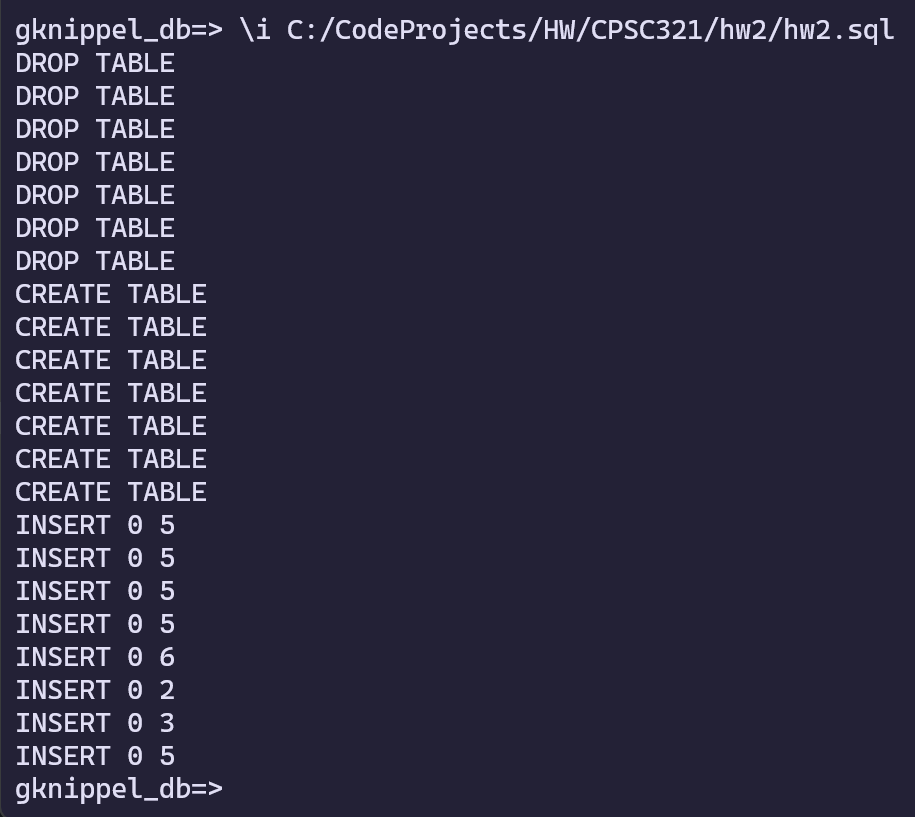
\includegraphics[width=0.55\textwidth]{scriptSuccess.png}
\end{figure}

\section*{table contents}

\begin{figure}[H]
\centering
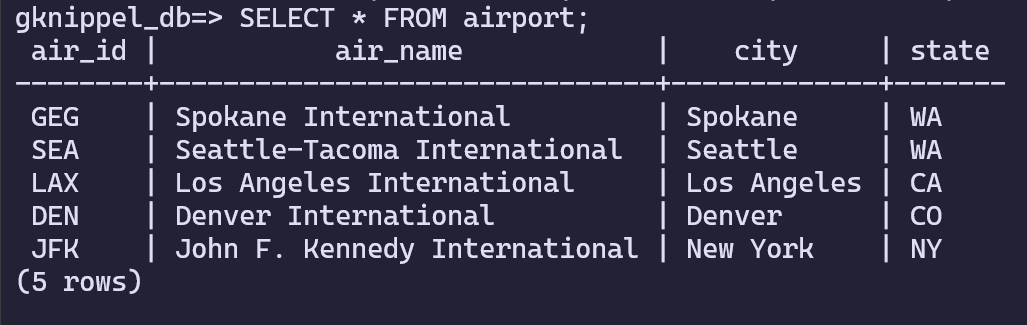
\includegraphics[width=\textwidth]{airport.png}\\[10pt]
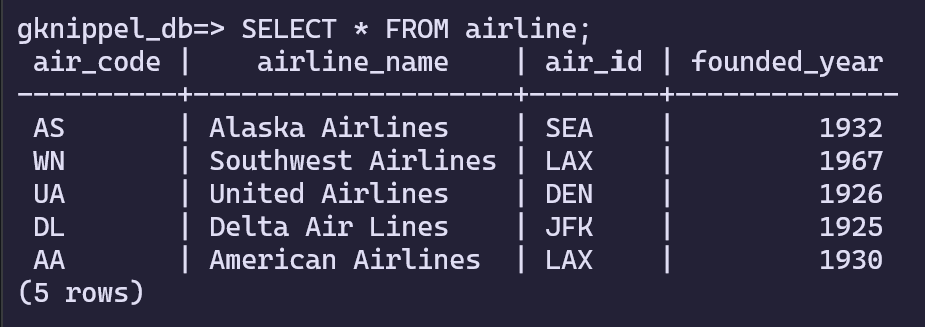
\includegraphics[width=\textwidth]{airline.png}\\[10pt]
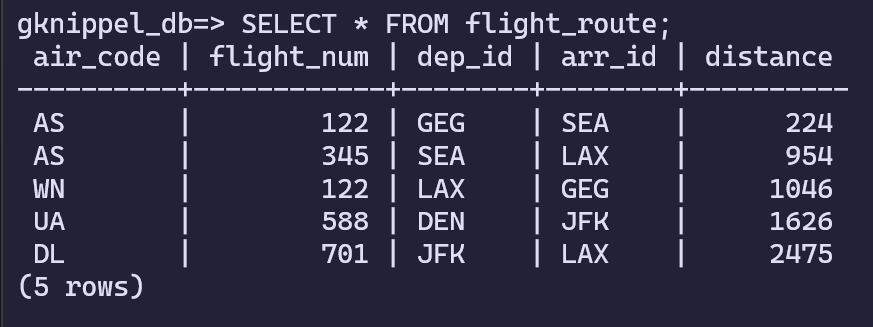
\includegraphics[width=\textwidth]{flight_route.png}
\end{figure}

\begin{figure}[H]
\centering
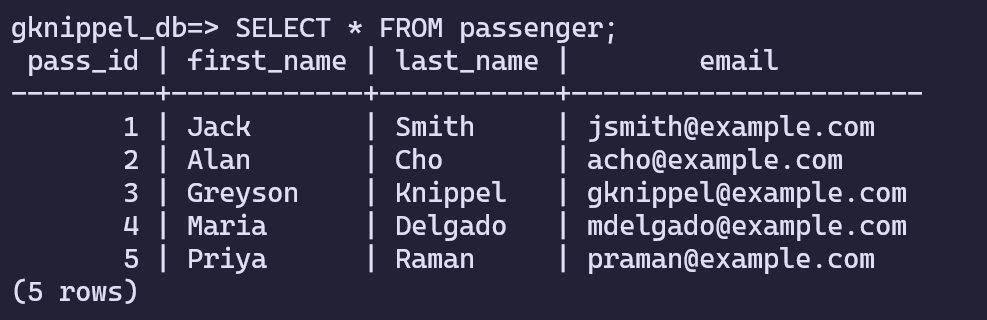
\includegraphics[width=\textwidth]{passenger.png}\\[10pt]
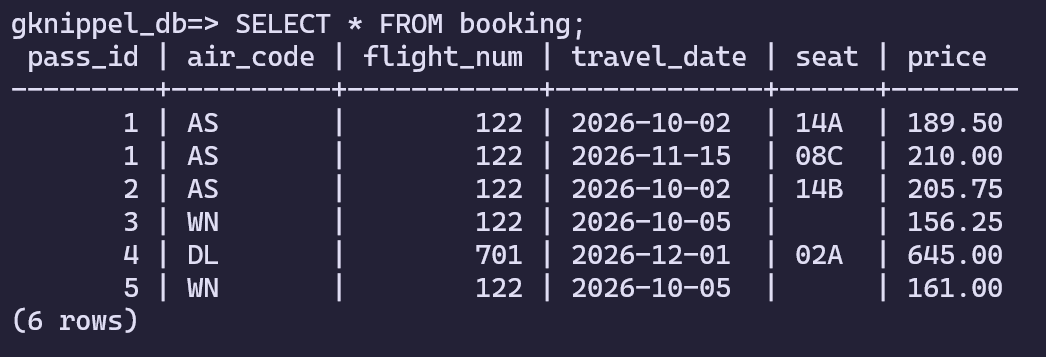
\includegraphics[width=\textwidth]{booking.png}
\end{figure}

\begin{figure}[H]
\centering
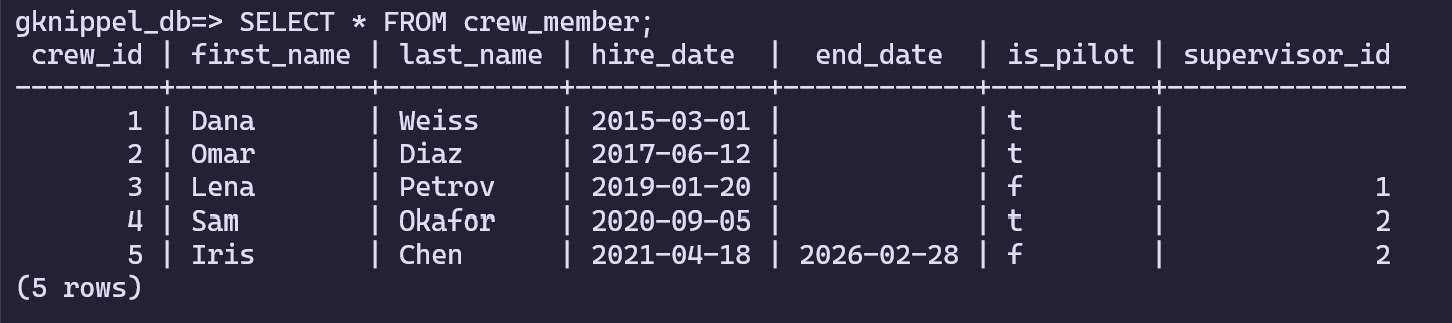
\includegraphics[width=\textwidth]{crew_member.png}\\[10pt]
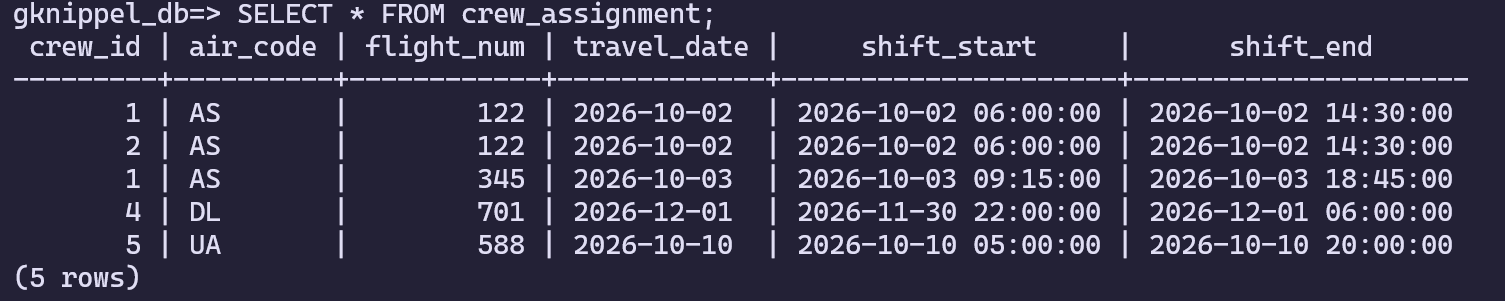
\includegraphics[width=\textwidth]{crew_assignment.png}
\end{figure}

\section*{failing inserts}

each statement below is commented out in the sql file. 

\subsection*{1. duplicate primary key}

duplicate primary key: 'GEG' is already the primary key of an existing airport row.

\begin{figure}[H]
\centering
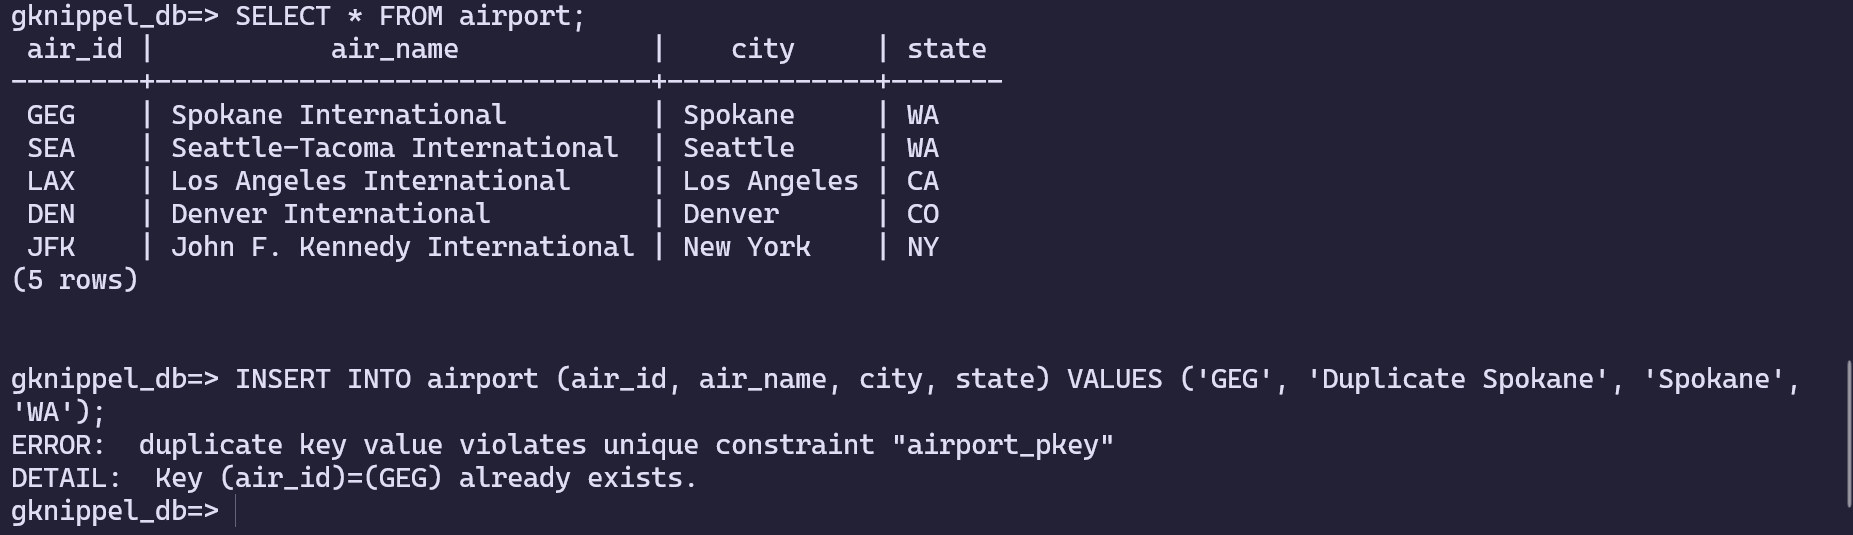
\includegraphics[width=\textwidth]{ss1.png}
\end{figure}

\subsection*{2. foreign-key violation}

foreign key violating: hub airport 'XXX' does not exist in airport.

\begin{figure}[H]
\centering
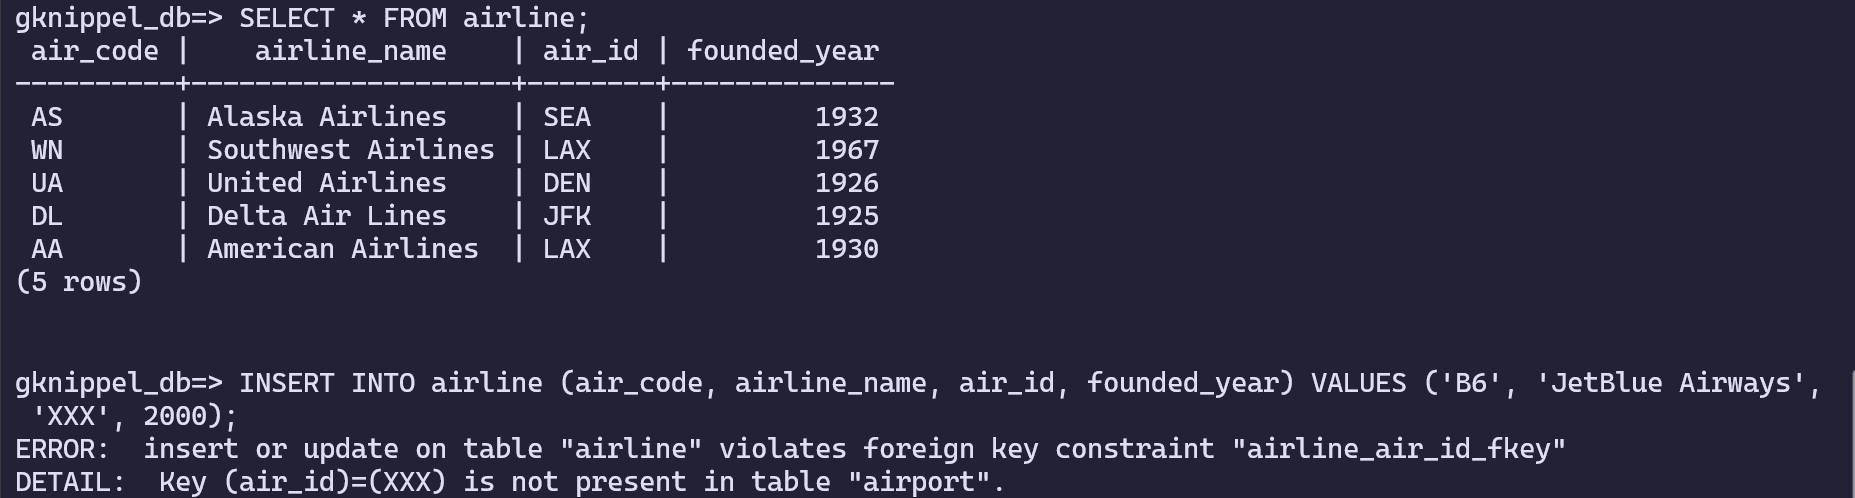
\includegraphics[width=\textwidth]{ss2.png}
\end{figure}

\subsection*{3. NOT NULL violation}

non null violation: email cant be NOT NULL.


\begin{figure}[H]
\centering
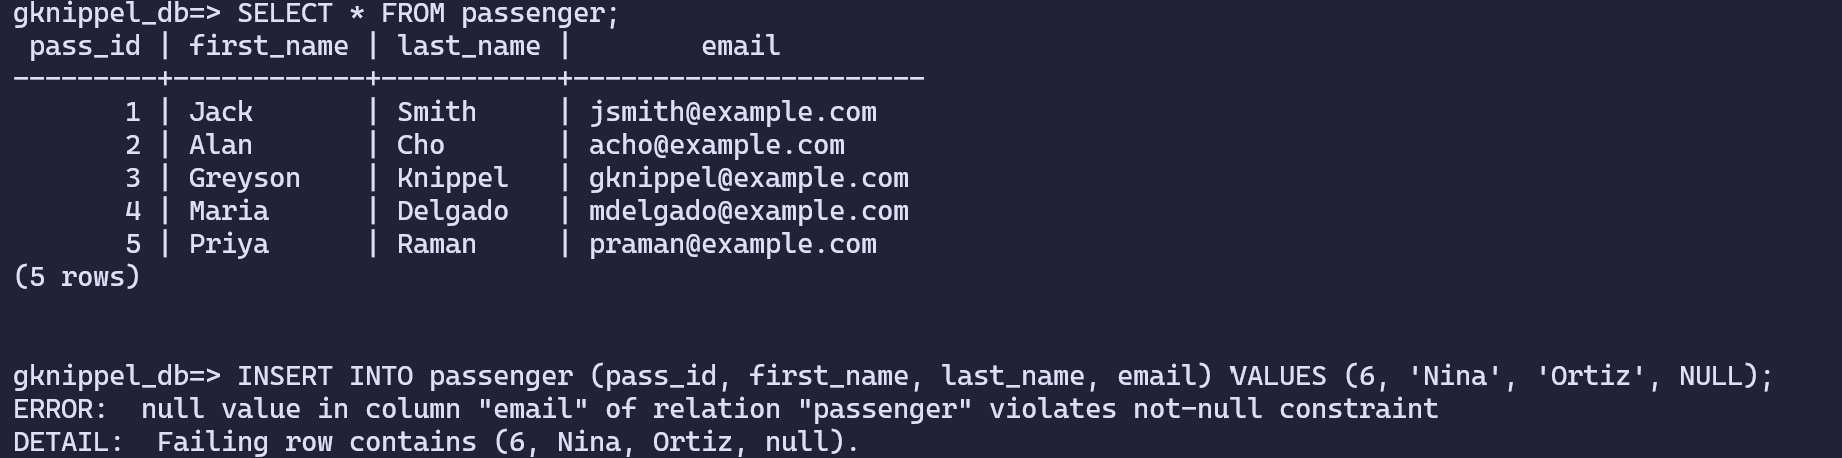
\includegraphics[width=\textwidth]{ss3.png}
\end{figure}

\subsection*{4. CHECK violation - departure equals arrival}

check violation: departure and arrival airports must be different.

\begin{figure}[H]
\centering
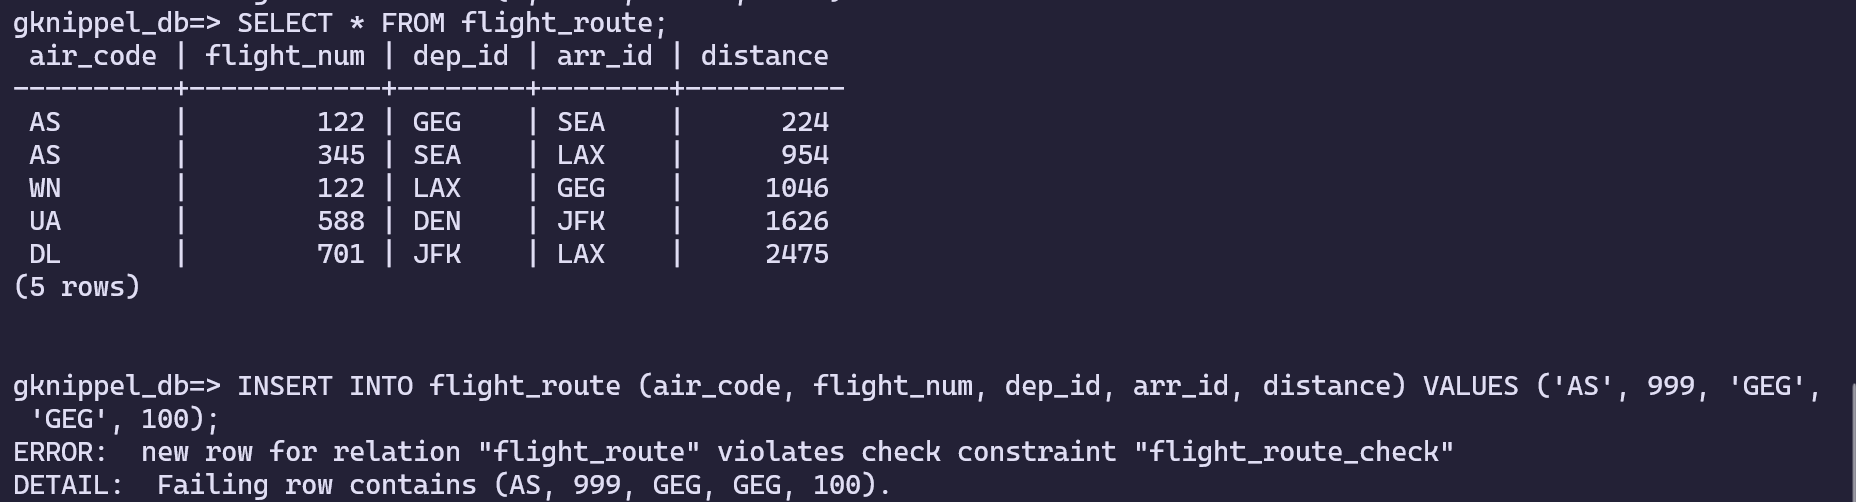
\includegraphics[width=\textwidth]{ss4.png}
\end{figure}

\subsection*{5. CHECK - negative price}

check violation: booking price cant be negative.

\begin{figure}[H]
\centering
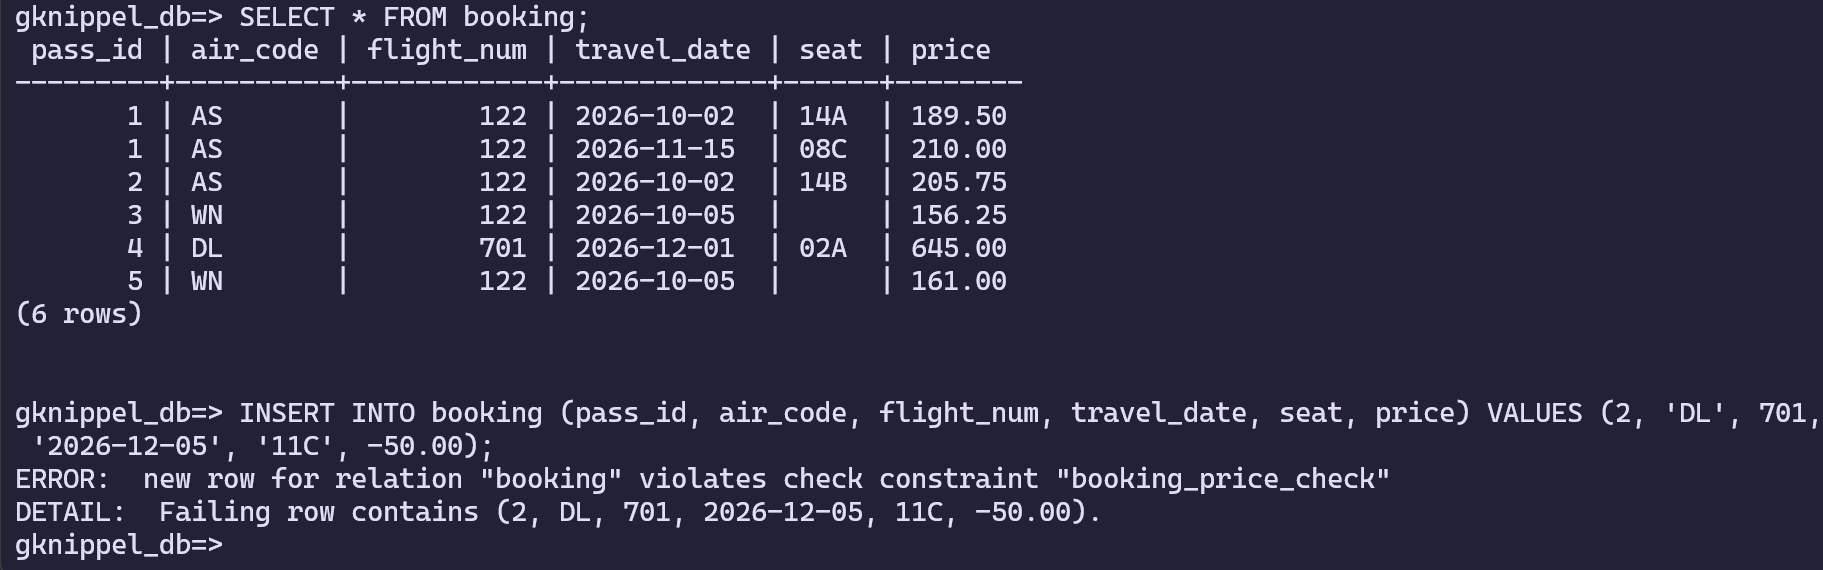
\includegraphics[width=\textwidth]{ss5.png}
\end{figure}

\subsection*{6. UNIQUE violation - duplicate email}

unique violation: (not the primary key): email is a candidate key, and this address already belongs to passenger 1.

\begin{figure}[H]
\centering
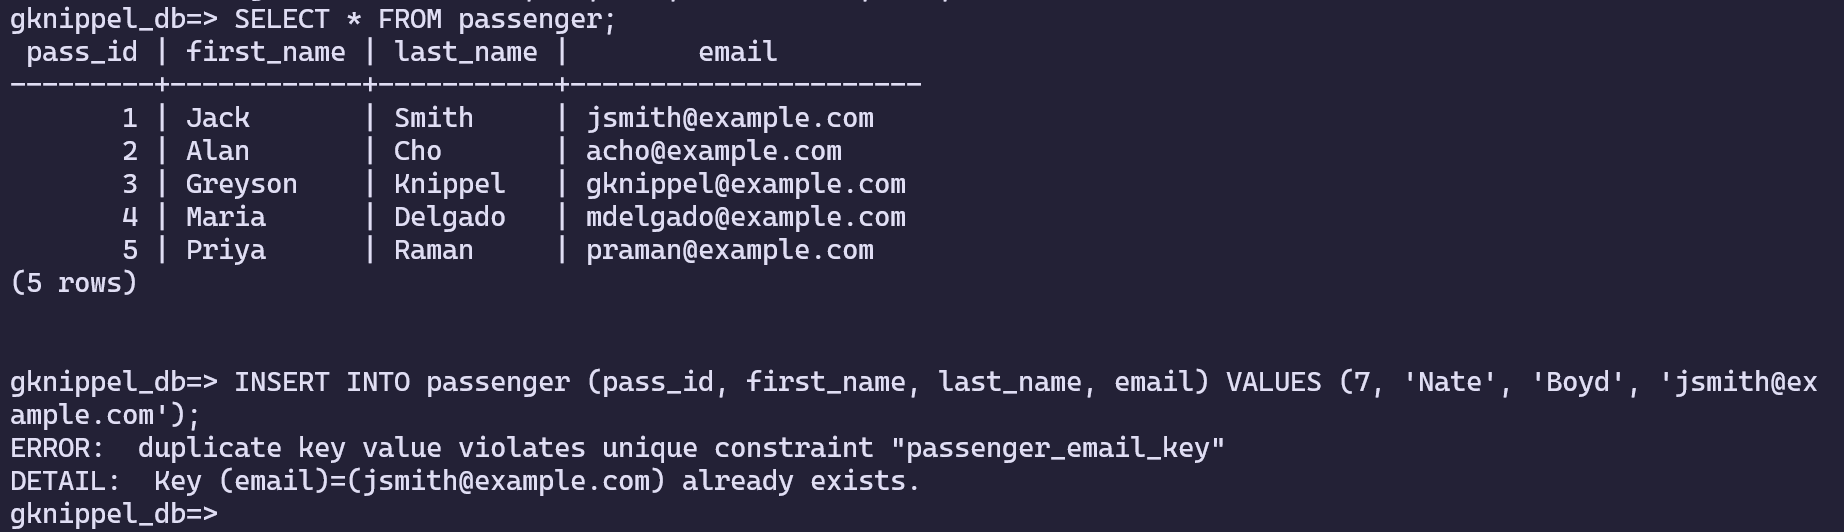
\includegraphics[width=\textwidth]{ss6.png}
\end{figure}

\subsection*{7. UNIQUE violation - seat already held}

unique violation: (not the primary key): seat 14A on AS 122 for 2026-10-02 is already taken by another passenger.

\begin{figure}[H]
\centering
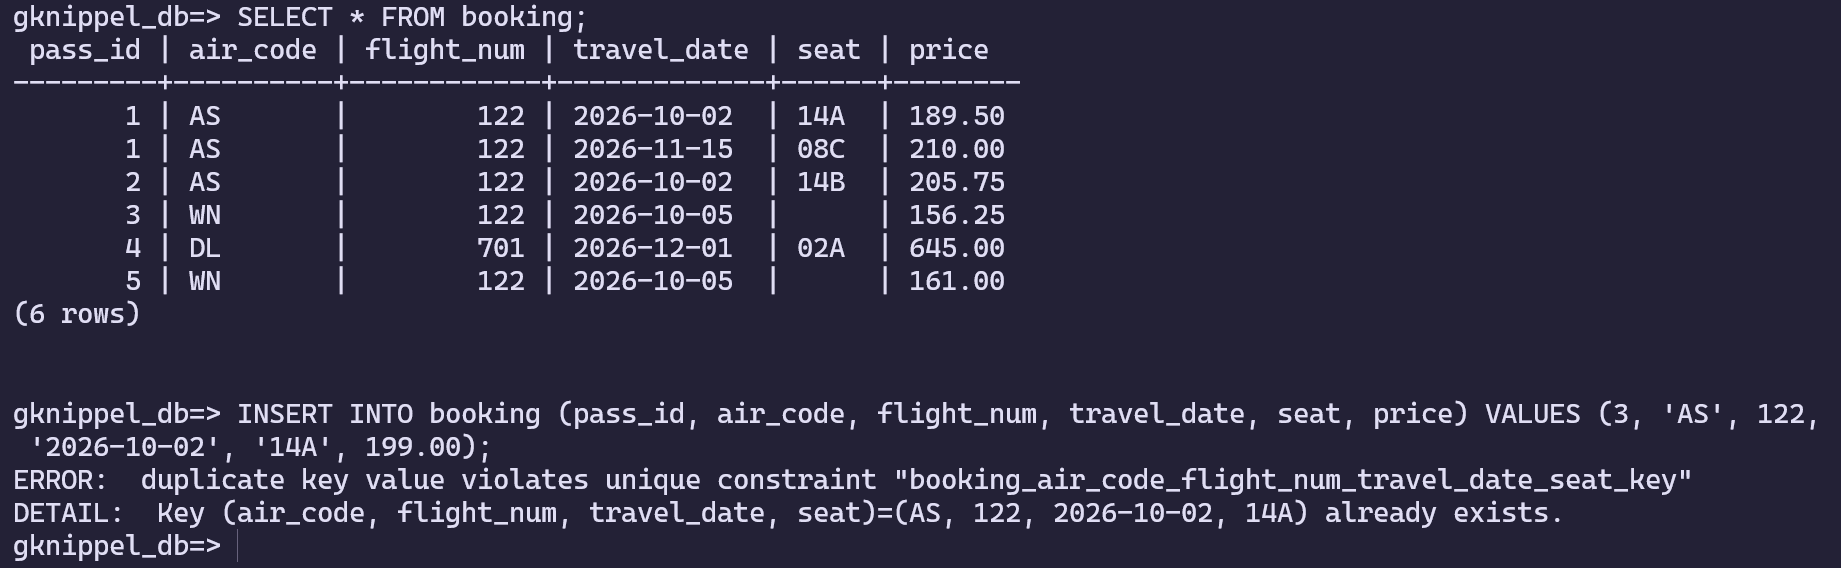
\includegraphics[width=\textwidth]{ss7.png}
\end{figure}

\section*{extra notes on the design}

this implementation follows the part A design from hw1 without drastic
change. all the tables, primary keys, and foreign keys are the same; the work in
this assignment was mostly the data types and constraints.

\end{document}
